% ========================================
% Chapitre 5 : Modèle binomial multi-périodes et options américaines
% ========================================
\chapter{Modèle binomial multi-périodes et options américaines}

\section{Modèle binomial multi-périodes ($T=3$)}

Considérons un modèle binomial à $T=3$ périodes.  
La filtration est donnée par $(\mathcal{J}_t)_{t=0,\dots,3}$ avec :
\[
\mathcal{J}_0=\{\emptyset,\Omega\},\quad
\mathcal{J}_1=\sigma(A_1,A_2),\quad
\mathcal{J}_2=\sigma(B_1,B_2,B_3,B_4),\quad
\mathcal{J}_3=\mathcal{P}(\Omega),
\]
où
\begin{itemize}
    \item $A_1 = \{\omega \in \Omega : \omega_1 = u\}$,
    \item $A_2 = \{\omega \in \Omega : \omega_1 = d\}$,
    \item $B_1 = \{\omega : \omega_1 = u,\ \omega_2 = u\}$,
    \item $B_2 = \{\omega : \omega_1 = u,\ \omega_2 = d\}$,
    \item $B_3 = \{\omega : \omega_1 = d,\ \omega_2 = u\}$,
    \item $B_4 = \{\omega : \omega_1 = d,\ \omega_2 = d\}$.
\end{itemize}

On considère un actif sans risque (obligation) de prix $S_t^0 = e^{rt}$  
et un actif risqué (action) de prix $S_t^1$.

L'évolution du prix de l'action peut être représentée par un arbre binaire :

\begin{figure}[H]
\centering
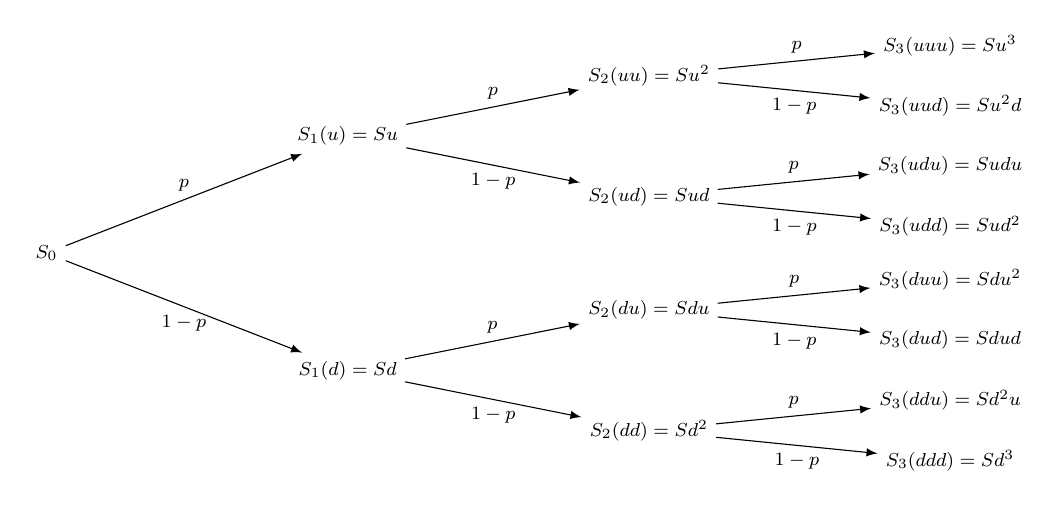
\begin{tikzpicture}[
    grow=right,
    scale=0.85, transform shape,
    level distance=45mm,
    level 1/.style={sibling distance=35mm},
    level 2/.style={sibling distance=18mm},
    level 3/.style={sibling distance=9mm},
    every node/.style={align=center, font=\footnotesize},
    edge from parent/.style={draw, -latex, thin},
    edge label/.style={font=\scriptsize, inner sep=1pt, sloped, above}
]

\node {$S_0$}
    child {
        node {$S_1(d)=Sd$}
        child {
            node {$S_2(dd)=Sd^2$}
            child {
                node {$S_3(ddd)=Sd^3$}
                edge from parent node[below] {$1-p$}
            }
            child {
                node {$S_3(ddu)=Sd^2u$}
                edge from parent node[above] {$p$}
            }
            edge from parent node[below] {$1-p$}
        }
        child {
            node {$S_2(du)=Sdu$}
            child {
                node {$S_3(dud)=Sdud$}
                edge from parent node[below] {$1-p$}
            }
            child {
                node {$S_3(duu)=Sdu^2$}
                edge from parent node[above] {$p$}
            }
            edge from parent node[above] {$p$}
        }
        edge from parent node[below] {$1-p$}
    }
    child {
        node {$S_1(u)=Su$}
        child {
            node {$S_2(ud)=Sud$}
            child {
                node {$S_3(udd)=Sud^2$}
                edge from parent node[below] {$1-p$}
            }
            child {
                node {$S_3(udu)=Sudu$}
                edge from parent node[above] {$p$}
            }
            edge from parent node[below] {$1-p$}
        }
        child {
            node {$S_2(uu)=Su^2$}
            child {
                node {$S_3(uud)=Su^2d$}
                edge from parent node[below] {$1-p$}
            }
            child {
                node {$S_3(uuu)=Su^3$}
                edge from parent node[above] {$p$}
            }
            edge from parent node[above] {$p$}
        }
        edge from parent node[above] {$p$}
    };
\end{tikzpicture}

\caption{Évolution du prix de l'action dans un modèle binomial à 3 périodes.}
\end{figure}

\section{Absence d'arbitrage et mesure risque-neutre}

La condition de non-arbitrage (NA) dans le modèle à $T=3$ équivaut à sa validité dans chaque sous-modèle à une période.  
Dans le cas binomial, elle s'écrit :
\begin{equation}
d < e^r < u.
\end{equation}

L'existence d'une mesure de martingale équivalente (EMM) $Q$ est équivalente à (NA).  
Sous $Q$, le prix actualisé de l'action est une martingale :
\begin{equation}
\E_Q[\hat{S}_{t+1} \mid \mathcal{J}_t] = \hat{S}_t,
\end{equation}
où $\hat{S}_t = S_t / S_t^0 = e^{-rt} S_t$.

Pour tout nœud $(\omega_1, \dots, \omega_t)$, on a :
\[
e^{-rt} S_t(\omega_1, \dots, \omega_t)
= \E_Q[e^{-r(t+1)} S_{t+1} \mid \mathcal{J}_t],
\]
soit encore :
\[
S_t = e^{-r} \left[ S_{t+1}(u)\, Q_{(\omega_1,\dots,\omega_t)}(u)
+ S_{t+1}(d)\, Q_{(\omega_1,\dots,\omega_t)}(d) \right].
\]

Résolvons pour un nœud particulier, par exemple $t=2$ après deux hausses :
\[
S_2(uu) = e^{-r} \big[S_3(uuu)\, q_{uu} + S_3(uud)\,(1-q_{uu})\big],
\]
soit
\[
S u^2 = e^{-r} \big[S u^3 q_{uu} + S u^2 d (1-q_{uu})\big].
\]
On obtient alors
\[
1 = e^{-r}\,[u q_{uu} + d(1-q_{uu})]
\quad\Rightarrow\quad
e^r = d + (u-d) q_{uu},
\]
d'où la probabilité risque-neutre :
\[
q_{uu} = q = \frac{e^r - d}{u - d}, \qquad
1-q_{uu} = \frac{u - e^r}{u - d}.
\]
Dans ce modèle, les rendements sont indépendants du chemin, donc la probabilité $q$ est la même à chaque nœud.

\section{Valorisation et couverture d'une créance contingente}

Pour valoriser une créance contingente de payoff $B$ à l'échéance $T=3$, on utilise la formule d'évaluation sous la mesure risque-neutre :
\begin{equation}
A_t = \E_Q[B \mid \mathcal{J}_t],
\end{equation}
où $A_t$ désigne le prix de la créance à la date $t$.

Pour couvrir la créance, on construit un portefeuille auto-financé $(H_t^0,H_t^1)$ tel que sa valeur coïncide avec celle de la créance à chaque date.  
La composition du portefeuille est donnée par :
\begin{align}
H_t^1 &= \frac{A_{t+1}(u) - A_{t+1}(d)}{S_{t+1}(u) - S_{t+1}(d)}
\quad &\text{(nombre d'actions détenues)}\\
H_t^0 &= e^{-r}\,\big(A_{t+1}(u) - H_t^1 S_{t+1}(u)\big)
\quad &\text{(montant investi dans l'actif sans risque).}
\end{align}
Comme le marché est complet, la mesure $Q$ est unique et toute créance peut être parfaitement répliquée.

\section*{Exemple numérique : Modèle binomial}

Paramètres : $T=3$, $u=1.1$, $d=0.9$, $r=\log(1+0.05)$, $S_0=20$

\subsection*{Arbre des prix de l'action}

\begin{center}
\begin{tikzpicture}[scale=0.85, transform shape]
    % Node styles
    \tikzstyle{n} = [align=center, font=\small]
    
    % Nodes
    % t=0
    \node[n] (n0) at (0,0) {20};
    
    % t=1
    \node[n] (n1u) at (3, 1.5) {22 \\ \textcolor{red}{(20.95)}};
    \node[n] (n1d) at (3, -1.5) {18 \\ \textcolor{red}{(17.14)}};
    
    % t=2
    \node[n] (n2uu) at (6, 3) {24.2 \\ \textcolor{red}{(21.95)}};
    \node[n] (n2ud) at (6, 0) {19.8 \\ \textcolor{red}{(17.96)}};
    \node[n] (n2dd) at (6, -3) {16.2 \\ \textcolor{red}{(14.69)}};
    
    % t=3
    \node[n] (n3uuu) at (9, 4.5) {26.62 \\ \textcolor{red}{(23)}};
    \node[n] (n3uud) at (9, 1.5) {21.78 \\ \textcolor{red}{(18.81)}};
    \node[n] (n3udd) at (9, -1.5) {17.82 \\ \textcolor{red}{(15.39)}};
    \node[n] (n3ddd) at (9, -4.5) {14.58 \\ \textcolor{red}{(12.59)}};
    
    % Edges
    \draw[->] (n0) -- (n1u);
    \draw[->] (n0) -- (n1d);
    
    \draw[->] (n1u) -- (n2uu);
    \draw[->] (n1u) -- (n2ud);
    \draw[->] (n1d) -- (n2ud);
    \draw[->] (n1d) -- (n2dd);
    
    \draw[->] (n2uu) -- (n3uuu);
    \draw[->] (n2uu) -- (n3uud);
    \draw[->] (n2ud) -- (n3uud);
    \draw[->] (n2ud) -- (n3udd);
    \draw[->] (n2dd) -- (n3udd);
    \draw[->] (n2dd) -- (n3ddd);

\end{tikzpicture}
\end{center}

\vspace{1cm}

\noindent Notation: $\hat{S}_t$ and $\left(\hat{S}_t^1\right)$

\vspace{1cm}

\subsection*{Prix d'un Put Européen avec $K=20$ et $T=3$}

$$\hat{B} = \left(-\hat{S}_T + K\right)_+ \quad \text{avec} \quad K \cdot e^{-3r} \approx 17.28 \text{ (valeur actualisée du strike)}$$

\newpage

\subsection*{Probabilités Risque-Neutre}

Ici $Q_{(w_1,w_2)}(w_u) = Q_{w_1}(w_u) = Q(w_u) = \frac{3}{4}$

$Q_{(w_1,w_2)}(w_d) = Q_{w_1}(w_d) = Q(w_d) = \frac{1}{4}$

\vspace{0.5cm}

$$B = \left(\frac{K}{e^{3r}} - S_3^1\right)_+ = A_3 = \begin{cases}
0 \\
0 \\
1.89 \\
4.69
\end{cases}$$

où $e^{3r} = 17.28$

\subsection*{Arbre pour $A_t$ (Prix de l'option)}

L'arbre binomial suivant représente le prix de l'option de vente européenne à chaque nœud. Les nœuds sont numérotés de \circled{1} à \circled{6} et les valeurs actualisées des payoffs terminaux ($A_3$) sont indiquées à droite.

\begin{center}
\begin{center}
\begin{tikzpicture}[scale=0.85, transform shape]
    % Node styles
    \tikzstyle{n} = [circle, draw, minimum size=0.9cm, font=\small, fill=white]
    \tikzstyle{l} = [font=\small, align=left]

    % Coordinates for Recombining Tree
    % t=0
    \node[n] (n1) at (0,0) {\circled{1}};
    
    % t=1
    \node[n] (n3) at (3, 1.5) {\circled{3}};
    \node[n] (n2) at (3, -1.5) {\circled{2}};
    
    % t=2
    \node[n] (n6) at (6, 3) {\circled{6}};
    \node[n] (n5) at (6, 0) {\circled{5}};
    \node[n] (n4) at (6, -3) {\circled{4}};
    
    % t=3 (Leaves/Payoffs)
    \node[right] at (8, 4.5) {0};
    \node[right] at (8, 1.5) {0};
    \node[right] at (8, -1.5) {1.89};
    \node[right] at (8, -4.5) {4.69};
    
    % Edges
    % t=0 -> t=1
    \draw[->, thick] (n1) -- (n3);
    \draw[->, thick] (n1) -- (n2);
    
    % t=1 -> t=2
    \draw[->, thick] (n3) -- (n6);
    \draw[->, thick] (n3) -- (n5);
    \draw[->, thick] (n2) -- (n5);
    \draw[->, thick] (n2) -- (n4);
    
    % t=2 -> t=3 (Payoff links)
    \draw[->] (n6) -- (7.5, 4.5);
    \draw[->] (n6) -- (7.5, 1.5);
    \draw[->] (n5) -- (7.5, 1.5);
    \draw[->] (n5) -- (7.5, -1.5);
    \draw[->] (n4) -- (7.5, -1.5);
    \draw[->] (n4) -- (7.5, -4.5);

\end{tikzpicture}
\end{center}
\end{center}

\begin{center}
\underline{Payoff actualisé}
\end{center}

\textbf{Calcul rétrograde des $A_t$ :} On remonte l'arbre en calculant l'espérance actualisée sous $Q$ (avec $q = 3/4$) :

\begin{align*}
\circled{6} &= q \times 0 + (1-q) \times 0 = 0 \\
\circled{5} &= q \times 0 + (1-q) \times 1.89 \approx 0.47 \\
\circled{4} &= q \times 1.89 + (1-q) \times 4.69 \approx 2.58 \\[1em]
\circled{3} &= q \times \circled{6} + (1-q) \times \circled{5} \approx 0.12 \\
\circled{2} &= q \times \circled{5} + (1-q) \times \circled{4} \approx 1.00 \\[1em]
\circled{1} &= q \times \circled{3} + (1-q) \times \circled{2} \approx 0.34
\end{align*}

\newpage

\subsection*{Arbre pour $\textcolor{teal}{H_t^0}$ et $\textcolor{red}{H_t^1}$}

L'arbre suivant montre les valeurs de la stratégie de couverture à chaque nœud. Les nœuds en \textcolor{teal}{cyan} représentent $H^0$ (position en actif sans risque) et les nœuds en \textcolor{red}{rouge} représentent $H^1$ (Delta, position en actif risqué).

\begin{center}
\begin{center}
\begin{center}
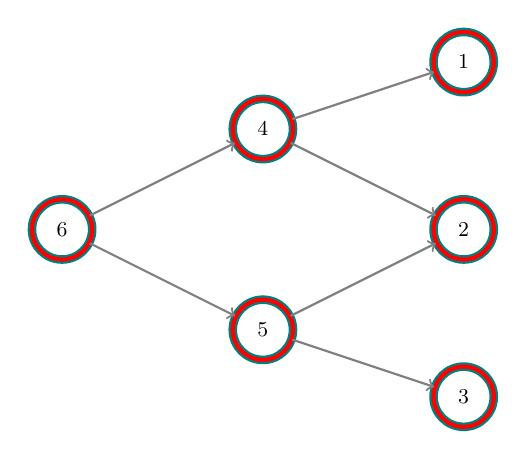
\begin{tikzpicture}[scale=0.85, transform shape]
    % Node styles
    % Double circle to represent both H^0 (teal) and H^1 (red)
    \tikzstyle{n} = [circle, draw=teal, double=red, double distance=1.5pt, minimum size=0.9cm, font=\small, fill=white, thick]
    
    % Tree Layout (Non-recombining for Strategy as per notes)
    % t=0
    \node[n] (n6) at (0,0) {\circled{6}};
    
    % t=1
    \node[n] (n4) at (3, 1.5) {\circled{4}};
    \node[n] (n5) at (3, -1.5) {\circled{5}};
    
    % t=2
    \node[n] (n1) at (6, 2.5) {\circled{1}}; % UU
    \node[n] (n2) at (6, 0) {\circled{2}}; % UD/DU (Recombining)
    \node[n] (n3) at (6, -2.5) {\circled{3}}; % DD
    
    % Edges
    \draw[->, thick, gray] (n6) -- (n4);
    \draw[->, thick, gray] (n6) -- (n5);
    
    \draw[->, thick, gray] (n4) -- (n1);
    \draw[->, thick, gray] (n4) -- (n2);
    
    \draw[->, thick, gray] (n5) -- (n2);
    \draw[->, thick, gray] (n5) -- (n3);

\end{tikzpicture}
\end{center}
\end{center}
\end{center}

\subsection*{Par exemple}

\textbf{Calcul de $H_2^1(w_u, w_u)$ :}
\[
\circled{3} = H_2^1(w_u, w_u) = \frac{A_3(w_u, w_u, w_u) - A_3(w_u, w_u, w_d)}{S_3^1(w_u, w_u, w_u) - S_3^1(w_u, w_u, w_d)} = -1
\]

\textbf{Calcul de $H_2^0(w_u, w_u)$ :} (actif finançant)
\[
\circled{3} = H_2^0(w_u, w_u) = A_2(w_u, w_u) - H_2^1(w_u, w_u) \times S_2^1(w_u, w_u) = 17.27
\]

\subsection*{De la même manière}

\begin{minipage}{0.45\textwidth}
\textbf{Valeurs de $\textcolor{teal}{H^0}$ :}
\begin{align*}
\textcolor{teal}{\circled{1}} &= 0 \\
\textcolor{teal}{\circled{2}} &= 10.35 \\
\textcolor{teal}{\circled{4}} &= 2.634 \\
\textcolor{teal}{\circled{5}} &= 11.95 \\
\textcolor{teal}{\circled{6}} &= 4.44
\end{align*}
\end{minipage}
\hfill
\begin{minipage}{0.45\textwidth}
\textbf{Valeurs de $\textcolor{red}{H^1}$ :}
\begin{align*}
\textcolor{red}{\circled{1}} &= 0 \\
\textcolor{red}{\circled{2}} &= -0.55 \\
\textcolor{red}{\circled{3}} &= -1 \\
\textcolor{red}{\circled{4}} &= -0.12 \\
\textcolor{red}{\circled{5}} &= -0.64 \\
\textcolor{red}{\circled{6}} &= -0.23
\end{align*}
\end{minipage}

\section{Options américaines}

\subsection{Définition}

Une option américaine est un processus stochastique non négatif $(\hat{X}_t)_{t=0,\dots,T}$ adapté à la filtration $(\mathcal{J}_t)$, que le détenteur peut exercer à tout instant $t\in\{0,\dots,T\}$ pour recevoir le paiement $\hat{X}_t$.

\begin{itemize}
    \item Option d'achat américaine (call) : $\hat{X}_t = (S_t - K)_+$,
    \item Option de vente américaine (put) : $\hat{X}_t = (K - S_t)_+$.
\end{itemize}

Dans un marché complet, on ne peut pas répliquer parfaitement une option américaine par une stratégie statique, car la date d'exercice est aléatoire.

\subsection{Valorisation par récurrence rétrograde}

Soit $(\hat{U}_t)_{t=0,\dots,T}$ le processus de prix d'une option américaine.  
À maturité : $\hat{U}_T = \hat{X}_T$.  
À la date $T-1$, le détenteur choisit entre :
\begin{enumerate}
    \item exercer et recevoir $\hat{X}_{T-1}$ ;
    \item ne pas exercer et conserver une option valant
    $\E_Q[e^{-r}\hat{X}_T \mid \mathcal{J}_{T-1}]$.
\end{enumerate}
Ainsi :
\[
\hat{U}_{T-1} = \max\!\left(\hat{X}_{T-1},\, \E_Q[e^{-r}\hat{U}_T\mid\mathcal{J}_{T-1}]\right),
\]
et, par récurrence, pour tout $t<T$ :
\[
\hat{U}_t = \max\!\left(\hat{X}_t,\, \E_Q[e^{-r}\hat{U}_{t+1}\mid\mathcal{J}_t]\right).
\]

En posant $U_t = e^{-rt}\hat{U}_t$ et $X_t = e^{-rt}\hat{X}_t$ (valeurs actualisées), on obtient :
\begin{equation}
U_t = \max\!\left(X_t,\, \E_Q[U_{t+1}\mid\mathcal{J}_t]\right).
\end{equation}

\begin{proposition}[Enveloppe de Snell]
Le processus actualisé $(U_t)$ est la plus petite sur-martingale sous $Q$ dominant le processus $(X_t)$.
\end{proposition}

\begin{proof}
La démonstration se fait en deux étapes :
\begin{enumerate}
    \item \textbf{$U$ domine $X$ et est une sur-martingale :}
    Par définition, $U_t = \max(X_t, \E_Q[U_{t+1}|\mathcal{J}_t])$.
    Donc $U_t \ge X_t$ (dominance).
    De plus, $U_t \ge \E_Q[U_{t+1}|\mathcal{J}_t]$ (sur-martingale).
    
    \item \textbf{$U$ est la plus petite :}
    Soit $(Y_t)$ une autre sur-martingale dominant $(X_t)$.
    À $t=T$, $U_T = X_T \le Y_T$.
    Supposons par récurrence que $U_{t+1} \le Y_{t+1}$.
    Alors, par la propriété de sur-martingale de $Y$ :
    \[
    \E_Q[U_{t+1}|\mathcal{J}_t] \le \E_Q[Y_{t+1}|\mathcal{J}_t] \le Y_t.
    \]
    De plus, par hypothèse de dominance, $X_t \le Y_t$.
    Par conséquent :
    \[
    U_t = \max(X_t, \E_Q[U_{t+1}|\mathcal{J}_t]) \le \max(Y_t, Y_t) = Y_t.
    \]
    Ainsi, $U_t \le Y_t$ pour tout $t$, ce qui prouve que $U$ est la plus petite sur-martingale dominante.
\end{enumerate}
\end{proof}

\begin{proposition}[Non-optimalité de l'exercice anticipé d'un Call]
Si le taux sans risque est non négatif ($S_t^0$ croissant), il n'est jamais optimal d'exercer une option d'achat américaine sur un titre sans dividendes avant l'échéance.
\end{proposition}

\begin{proof}[Preuve détaillée]
Nous cherchons à prouver qu'il n'est jamais optimal d'exercer une option d'achat américaine avant sa maturité $T$, à condition que le taux d'intérêt $r$ soit positif. Nous raisonnons par l'absurde.

\begin{enumerate}
    \item \textbf{Hypothèse par l'absurde :} Supposons qu'il existe un instant $t < T$ où l'exercice est optimal. Cela signifie que la valeur obtenue en exerçant immédiatement, $S_t - K$ (valeur intrinsèque), est strictement supérieure à la valeur espérée si l'on garde l'option, $\E_Q[e^{-r} \hat{U}_{t+1} \mid \mathcal{J}_t]$ (valeur de continuation).
    \[
    S_t - K > \E_Q[e^{-r} \hat{U}_{t+1} \mid \mathcal{J}_t]
    \]
    
    \item \textbf{Minoration de la valeur future :} La valeur future de l'option, $\hat{U}_{t+1}$, est toujours au moins égale à sa valeur d'exercice intrinsèque $(S_{t+1} - K)_+$.
    \[
    \hat{U}_{t+1} \ge (S_{t+1} - K)_+ \ge S_{t+1} - K
    \]
    
    \item \textbf{Application de l'espérance :} Prenons l'espérance conditionnelle actualisée de cette inégalité :
    \[
    \E_Q[e^{-r} \hat{U}_{t+1} \mid \mathcal{J}_t] \ge \E_Q[e^{-r} (S_{t+1} - K) \mid \mathcal{J}_t]
    \]
    
    \item \textbf{Propriété de Martingale :} Le terme de droite se développe par linéarité :
    \[
    \E_Q[e^{-r} S_{t+1} \mid \mathcal{J}_t] - e^{-r} K
    \]
    Sous la mesure $Q$, le prix actualisé $e^{-rt} S_t$ est une martingale. Donc $\E_Q[e^{-r(t+1)}S_{t+1} \mid \mathcal{J}_t] = e^{-rt}S_t$. En multipliant par $e^{rt}$, on a $\E_Q[e^{-r} S_{t+1} \mid \mathcal{J}_t] = S_t$.
    L'inégalité devient donc :
    \[
    \E_Q[e^{-r} \hat{U}_{t+1} \mid \mathcal{J}_t] \ge S_t - e^{-r} K
    \]
    
    \item \textbf{Contradiction :} Combinons l'hypothèse de départ (1) et le résultat (4) :
    \[
    S_t - K > \E_Q[e^{-r} \hat{U}_{t+1} \mid \mathcal{J}_t] \ge S_t - e^{-r} K
    \]
    En simplifiant par $S_t$, on obtient :
    \[
    -K > -e^{-r} K
    \]
    En multipliant par $-1$ (ce qui inverse l'inégalité) :
    \[
    K < e^{-r} K \iff K(1 - e^{-r}) < 0
    \]
    Or, si $r > 0$, alors $e^{-r} < 1$, donc $(1 - e^{-r}) > 0$. Puisque $K > 0$ également, le produit $K(1 - e^{-r})$ est \textbf{strictement positif}, ce qui contredit l'inégalité $K(1 - e^{-r}) < 0$.
    
    Cette contradiction montre que l'hypothèse initiale est fausse : il n'est jamais optimal d'exercer un call américain prématurément.
\end{enumerate}
\end{proof}

\subsection{Exemple Numérique : Option de Vente Américaine (Put)}
Reprenons le même modèle binomial que précédemment : $S_0=20, u=1.1, d=0.9, r=\ln(1.05)$, mais avec une option de vente américaine de strike $K=22$.

\begin{tcolorbox}[title=Arbre de Décision : Exercer ou Attendre ?, colback=blue!5!white, colframe=blue!50!black]
Les calculs se font à rebours. À chaque nœud, on compare la valeur intrinsèque $K-S_t$ avec la valeur de continuation.
\begin{itemize}
    \item $\mathbf{t=3}$ : Payoff $P_3 = (22 - S_3)_+$.
    \begin{itemize}
        \item $S_3(ddd) = 14.58 \implies P_3 = 7.42$
        \item $S_3(udd) = 17.82 \implies P_3 = 4.18$
        \item $S_3(uud) = 21.78 \implies P_3 = 0.22$
        \item $S_3(uuu) = 26.62 \implies P_3 = 0$
    \end{itemize}
    \item $\mathbf{t=2}$ : $P_2 = \max(22-S_2, e^{-r}[q P_3(u) + (1-q) P_3(d)])$.
    \begin{itemize}
        \item Nœud $dd$ ($S_2=16.2$) : Intrinsèque $= 5.8$. Continuation $\approx 4.75$. $\to$ \textbf{Exercice} (valeur 5.8).
        \item Nœud $ud$ ($S_2=19.8$) : Intrinsèque $= 2.2$. Continuation $\approx 1.15$. $\to$ \textbf{Exercice} (valeur 2.2).
        \item Nœud $uu$ ($S_2=24.2$) : Intrinsèque $= 0$. Continuation $\approx 0$. $\to$ Pas d'exercice.
    \end{itemize}
    \item $\mathbf{t=1}$ :
    \begin{itemize}
        \item Nœud $d$ ($S_1=18$) : Intrinsèque $= 4$. Continuation $\approx 2.95$. $\to$ \textbf{Exercice} (valeur 4).
        \item Nœud $u$ ($S_1=22$) : Intrinsèque $= 0$. Continuation $\approx 0.52$. $\to$ Pas d'exercice.
    \end{itemize}
    \item $\mathbf{t=0}$ ($S_0=20$) : Intrinsèque $= 2$. Continuation $\approx 1.32$. $\to$ \textbf{Exercice Immédiat} (valeur 2).
\end{itemize}
\end{tcolorbox}
Conclusion : Dans cet exemple spécifique, l'option de vente américaine a une valeur de 2 (exercice immédiat), nettement supérieure à celle de l'option européenne correspondante (qui vaudrait environ 1.32). Cela illustre la prime d'exercice anticipé.

\section{Temps d'arrêt et options américaines}

\begin{definition}[Temps d'arrêt]
Une variable aléatoire $\tau : \Omega \to \{0,\dots,T\}$ est un \emph{temps d'arrêt} si,
pour tout $t$, l'événement $\{\tau = t\}$ appartient à $\mathcal{J}_t$.
\end{definition}

\paragraph*{Intuition : Le Meilleur Moment pour Agir}
Le problème de la valorisation d'une option américaine est un exemple canonique de "problème d'arrêt optimal". Le détenteur de l'option est confronté à une série de décisions : à chaque instant $t$, doit-il exercer l'option et encaisser le gain $X_t$, ou doit-il attendre en espérant un gain futur plus élevé ? Un "temps d'arrêt" $\tau$ est une règle de décision qui ne dépend que du passé et du présent. Le détenteur cherche le temps d'arrêt optimal $\tau^*$ qui maximise l'espérance du gain actualisé, soit $\max_\tau \E_Q[X_\tau]$.

La formule de récurrence rétrograde que nous avons établie ($U_t = \max(X_t, \E_Q[U_{t+1} \mid \mathcal{J}_t])$) n'est autre que l'algorithme de programmation dynamique de Bellman qui résout ce problème d'arrêt optimal. À chaque étape, elle compare la valeur de l'action immédiate ("exercer maintenant") avec la valeur espérée de la stratégie optimale future ("continuer et prendre la meilleure décision plus tard"). Le processus $U_t$ représente donc la valeur maximale atteignable à partir de l'instant $t$.

Exercer une option américaine revient à choisir un temps d'arrêt $\tau$.  
Le gain obtenu est $X_\tau$.  
\begin{proof}
Nous devons montrer que le processus défini par $U_t = \sup_{\tau \in \mathcal{T}_t} \E_Q[X_\tau | \mathcal{J}_t]$ vérifie bien l'équation de récurrence de Bellman (Proposition 1).
Soit $V_t$ ce supremum.
À $t=T$, $V_T = X_T = U_T$.
Pour $t < T$, séparons l'ensemble des temps d'arrêt $\mathcal{T}_t$ en deux cas : $\tau = t$ (exercice immédiat) et $\tau > t$ (continuation).
Si $\tau > t$, alors $\tau$ est aussi un temps d'arrêt dans $\mathcal{T}_{t+1}$.
\[
V_t = \max \left( X_t, \sup_{\tau \in \mathcal{T}_{t+1}} \E_Q[X_\tau | \mathcal{J}_t] \right)
\]
En utilisant la propriété de tour (loi des espérances itérées) :
\[
\E_Q[X_\tau | \mathcal{J}_t] = \E_Q [ \E_Q[X_\tau | \mathcal{J}_{t+1}] | \mathcal{J}_t ]
\]
Donc :
\[
\sup_{\tau \in \mathcal{T}_{t+1}} \E_Q[X_\tau | \mathcal{J}_t] = \E_Q \left[ \sup_{\tau \in \mathcal{T}_{t+1}} \E_Q[X_\tau | \mathcal{J}_{t+1}] \mid \mathcal{J}_t \right] = \E_Q[V_{t+1} | \mathcal{J}_t]
\]
On retrouve ainsi :
\[
V_t = \max(X_t, \E_Q[V_{t+1} | \mathcal{J}_t])
\]
C'est exactement la relation de récurrence qui définit $(U_t)$. Par unicité, $U_t$ est bien le supremum des espérances de gains sur tous les temps d'arrêt possibles.
\end{proof}
